\documentclass[aspectratio=169]{beamer}

\usetheme{Boadilla}
\usefonttheme{professionalfonts}
\setbeamertemplate{navigation symbols}{}
\setbeamertemplate{itemize items}[circle]
\setbeamertemplate{enumerate items}[default]
\setbeamertemplate{headline}{}

\usepackage[utf8]{inputenc}
\usepackage[T1]{fontenc}
\usepackage{lmodern}
\usepackage{amsmath}
\usepackage{booktabs}
\usepackage{tabularx}
\usepackage{array}
\usepackage{hyperref}
\usepackage[strings]{underscore}
\usepackage{listings}
\usepackage{tikz}
\usetikzlibrary{arrows.meta,positioning,fit,calc,shapes.geometric}
\usepackage{xcolor}

\definecolor{courseblue}{HTML}{12355B}
\definecolor{coursegold}{HTML}{C98A2E}
\definecolor{courseice}{HTML}{EEF3F8}
\definecolor{coursegreen}{HTML}{2F6B4F}
\definecolor{coursegray}{HTML}{4B5563}
\definecolor{codebg}{HTML}{F7F9FC}
\definecolor{codecomment}{HTML}{5E6C84}
\definecolor{codestring}{HTML}{0B6E4F}

\setbeamercolor{palette primary}{bg=courseblue,fg=white}
\setbeamercolor{palette secondary}{bg=coursegold,fg=white}
\setbeamercolor{palette tertiary}{bg=courseblue,fg=white}
\setbeamercolor{palette quaternary}{bg=coursegold,fg=white}
\setbeamercolor{structure}{fg=courseblue}
\setbeamercolor{frametitle}{bg=courseice,fg=courseblue}
\setbeamercolor{title}{fg=courseblue}
\setbeamercolor{block title}{bg=courseblue,fg=white}
\setbeamercolor{block body}{bg=courseice,fg=black}
\setbeamercolor{normal text}{fg=black,bg=white}
\setbeamercolor{alerted text}{fg=coursegold}

\setbeamerfont{footline}{size=\scriptsize}

\setbeamertemplate{footline}{
  \leavevmode
  \hbox{
    \begin{beamercolorbox}[wd=.33\paperwidth,ht=2.8ex,dp=1.2ex,leftskip=0.8em]{palette primary}%
      University of Trieste
    \end{beamercolorbox}%
    \begin{beamercolorbox}[wd=.49\paperwidth,ht=2.8ex,dp=1.2ex,center]{palette tertiary}%
      \coursename{} \textbar{} \coursecode
    \end{beamercolorbox}%
    \begin{beamercolorbox}[wd=.18\paperwidth,ht=2.8ex,dp=1.2ex,rightskip=0.8em plus1fil]{palette secondary}%
      \insertframenumber{} / \inserttotalframenumber
    \end{beamercolorbox}%
  }
}

\hypersetup{
  colorlinks=true,
  linkcolor=courseblue,
  urlcolor=coursegreen
}

\lstdefinestyle{coursepython}{
  language=Python,
  basicstyle=\ttfamily\footnotesize,
  keywordstyle=\color{courseblue}\bfseries,
  commentstyle=\color{codecomment}\itshape,
  stringstyle=\color{codestring},
  showstringspaces=false,
  columns=fullflexible,
  keepspaces=true,
  frame=single,
  framerule=0.6pt,
  rulecolor=\color{courseblue},
  backgroundcolor=\color{codebg},
  xleftmargin=0.4em,
  xrightmargin=0.4em,
  aboveskip=0.4em,
  belowskip=0.2em
}

\newcommand{\coursename}{Data-driven Systems Engineering}
\newcommand{\coursecode}{440MI / 305SM}
\newcommand{\coursefooter}{}

\newcommand{\learninggoals}[1]{
  \begin{block}{Learning goals}
  #1
  \end{block}
}

\newcommand{\repoactivity}[1]{
  \begin{block}{Repo activity}
  #1
  \end{block}
}

\newcommand{\readinglist}[1]{
  \begin{block}{Papers and materials}
  {\footnotesize #1}
  \end{block}
}

\newcommand{\coursecontextframe}[5]{
  \begin{frame}{Course Map and Running Cases}
  \centering
  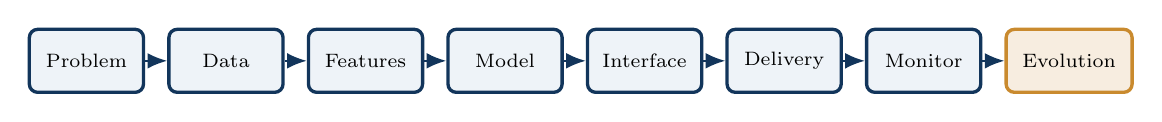
\begin{tikzpicture}[node distance=0.28cm]
  \node[flowbox, minimum width=1.45cm, minimum height=0.8cm] (problem) {\scriptsize Problem};
  \node[flowbox, minimum width=1.45cm, minimum height=0.8cm, right=of problem] (data) {\scriptsize Data};
  \node[flowbox, minimum width=1.45cm, minimum height=0.8cm, right=of data] (features) {\scriptsize Features};
  \node[flowbox, minimum width=1.45cm, minimum height=0.8cm, right=of features] (model) {\scriptsize Model};
  \node[flowbox, minimum width=1.45cm, minimum height=0.8cm, right=of model] (interface) {\scriptsize Interface};
  \node[flowbox, minimum width=1.45cm, minimum height=0.8cm, right=of interface] (delivery) {\scriptsize Delivery};
  \node[flowbox, minimum width=1.45cm, minimum height=0.8cm, right=of delivery] (monitor) {\scriptsize Monitor};
  \node[accentbox, minimum width=1.6cm, minimum height=0.8cm, right=of monitor] (evolution) {\scriptsize Evolution};
  \foreach \a/\b in {problem/data,data/features,features/model,model/interface,interface/delivery,delivery/monitor,monitor/evolution} {
    \draw[arrow] (\a) -- (\b);
  }
  \end{tikzpicture}

  \vspace{0.5em}
  \begin{block}{Today in the course}
  \textbf{Focus:} #1

  \textbf{Bridge:} #2
  \end{block}

  \begin{columns}[T]
  \column{0.48\textwidth}
  \begin{block}{Fraud case}
  {\footnotesize #3}
  \end{block}
  \column{0.48\textwidth}
  \begin{block}{Pasteurization case}
  {\footnotesize #4}
  \end{block}
  \end{columns}

  \vspace{0.3em}
  {\footnotesize \textbf{Course thread:} #5}
  \coursefooter
  \end{frame}
}

\newcommand{\classclosingframe}[4]{
  \begin{frame}{From This Class to the Next}
  \begin{block}{What stays with us}
  #1
  \end{block}

  \begin{columns}[T]
  \column{0.48\textwidth}
  \begin{block}{Project use}
  {\footnotesize #2}
  \end{block}
  \column{0.48\textwidth}
  \begin{block}{Next connection}
  {\footnotesize #3}
  \end{block}
  \end{columns}

  \vspace{0.3em}
  {\footnotesize \textbf{Course thread:} #4}
  \coursefooter
  \end{frame}
}

\tikzset{
  flowbox/.style={
    rounded corners=3pt,
    draw=courseblue,
    fill=courseice,
    very thick,
    minimum width=2.2cm,
    minimum height=0.9cm,
    align=center,
    font=\small
  },
  accentbox/.style={
    rounded corners=3pt,
    draw=coursegold,
    fill=coursegold!15,
    very thick,
    minimum width=2.2cm,
    minimum height=0.9cm,
    align=center,
    font=\small
  },
  arrow/.style={
    -{Latex[length=2.5mm,width=2mm]},
    thick,
    draw=courseblue
  }
}


\title{Class 13: Data Types and Structures for Data-Driven Systems}
\author{\coursename}
\date{}

\begin{document}

\frame{\titlepage \coursefooter}

\begin{frame}{Agenda}
\begin{itemize}
\item Why identifying data type comes before any modeling decision.
\item Tabular data: rows, columns, and the independence assumption.
\item Time series data: order, timestamps, and temporal dependency.
\item Spectral and signal data: waveforms and frequency-domain thinking.
\item Image data: pixels, grids, and spatial structure.
\item How the fraud and pasteurization cases embody different data types.
\end{itemize}
\coursefooter
\end{frame}

\begin{frame}{Learning goals}
\learninggoals{
\begin{itemize}
\item Recognize that ``a dataset'' is not one thing: tabular, time series, spectral, and image data carry different assumptions.
\item Identify which assumptions (independence, ordering, locality) each data type licenses or forbids.
\item Connect each data type to a concrete artifact already in this repository.
\item Explain why data type must be settled before encoding, feature engineering, or model choice.
\end{itemize}
}
\coursefooter
\end{frame}

\coursecontextframe
{Recognizing tabular, time series, spectral, and image data before any modeling begins.}
{This class opens the Data-Driven block: after twelve classes of Python fluency, we now slow down and ask what kind of data we actually have, before choosing how to represent or model it.}
{The fraud case is tabular: one row per transaction, columns of named or anonymized attributes, and no assumed order between rows.}
{The pasteurization case is a time series and signal problem: sensors sampled once per second, with heating and cooling dynamics that only make sense in temporal order.}
{Every later class (encoding, feature engineering, modeling, serving) depends on having correctly identified the data type first.}

\begin{frame}{Why data type matters before modeling}
\begin{itemize}
\item Algorithms encode implicit assumptions about structure: independence between rows, smoothness over time, or locality over space.
\item Using a tabular technique on ordered data can silently destroy the information that matters most (the order itself).
\item The same physical quantity, temperature, is tabular in one dataset and a time series in another, depending on how it was collected.
\item Choosing the right data type framing narrows down encoding, feature engineering, and model family choices dramatically.
\end{itemize}
\coursefooter
\end{frame}

\begin{frame}{Tabular data}
\begin{itemize}
\item Organized as rows (observations) and columns (variables), typically stored as a table, CSV file, or dataframe.
\item Rows are usually assumed independent and identically distributed (i.i.d.): shuffling rows should not change what a model can learn.
\item Columns can be numerical, categorical, or boolean, and each has a fixed meaning across all rows.
\item This is the default assumption behind most classical machine learning tooling.
\end{itemize}
\coursefooter
\end{frame}

\begin{frame}[fragile]{Tabular example: the fraud dataset}
\begin{lstlisting}[style=coursepython]
rename_map = {
    'Time': 'transaction_time',
    'Amount': 'transaction_amount',
    'Class': 'is_fraud'
}
for i in range(1, 29):
    rename_map[f'V{i}'] = f'V{i}_feature'
df.rename(columns=rename_map, inplace=True)
\end{lstlisting}
\begin{itemize}
\item This is from `Credit_Card_Fraud_Detection_Solution.ipynb`: one row per transaction, one named column per attribute.
\item Nothing in the fraud table depends on which row came before it; `transaction_time` is a column value, not a row ordering.
\end{itemize}
\coursefooter
\end{frame}

\begin{frame}{Four data types at a glance}
\begin{tabularx}{\textwidth}{>{\bfseries}l X}
Data type & Defining structure \\
\toprule
Tabular & Independent rows, fixed columns; order between rows carries no meaning. \\
Time series & Ordered samples over time; past values constrain and explain future ones. \\
Spectral / signal & A waveform best understood in the frequency domain, not only the time domain. \\
Image & A 2D (or 3D) grid of values where neighboring pixels are strongly correlated. \\
\bottomrule
\end{tabularx}
\coursefooter
\end{frame}

\begin{frame}{Time series data}
\begin{itemize}
\item Samples are ordered by timestamp, and that order is part of the data, not an artifact of storage.
\item Neighboring points are correlated: today's sensor reading depends on yesterday's process state.
\item Trends, seasonality, and regime changes (state transitions) are first-class phenomena.
\item Splitting or shuffling a time series naively for training and testing leaks future information into the past.
\end{itemize}
\coursefooter
\end{frame}

\begin{frame}[fragile]{Time series example: a pasteurization batch}
\begin{lstlisting}[style=coursepython]
def simulate_batch(bid, start_time=0.0):
    pdur = {k: int(rng.integers(*PROD_RANGES[k])) for k in PROD_RANGES}
    ...
    frames = simulate_production_cycle(pdur, ctx)
    df, t = to_df(frames, start_time, bid)
    df["dTdt"] = df["T"].diff().fillna(0.0) / DT
    return df, t
\end{lstlisting}
\begin{itemize}
\item `pasteurization/synth_sensors.py` generates one row per second, per sensor, for an entire batch lifecycle.
\item `dTdt` only makes sense because rows are ordered: it is a derivative with respect to time, computed with `.diff()`.
\end{itemize}
\coursefooter
\end{frame}

\begin{frame}{A time series is often also a state machine}
\centering
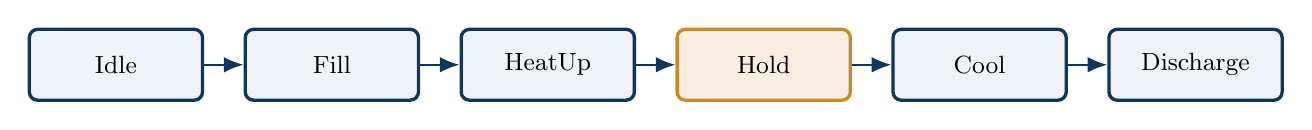
\begin{tikzpicture}[node distance=0.5cm]
\node[flowbox] (idle) {\small Idle};
\node[flowbox, right=of idle] (fill) {\small Fill};
\node[flowbox, right=of fill] (heat) {\small HeatUp};
\node[accentbox, right=of heat] (hold) {\small Hold};
\node[flowbox, right=of hold] (cool) {\small Cool};
\node[flowbox, right=of cool] (disch) {\small Discharge};
\foreach \a/\b in {idle/fill,fill/heat,heat/hold,hold/cool,cool/disch} {
  \draw[arrow] (\a) -- (\b);
}
\end{tikzpicture}
\vspace{0.6em}
\begin{itemize}
\item These are exactly the six states used by `PROD_RANGES` in `synth_sensors.py`.
\item Knowing the current state changes what a ``normal'' sensor reading looks like at that moment.
\end{itemize}
\coursefooter
\end{frame}

\begin{frame}{Stream example: from raw signal to derived feature}
\centering
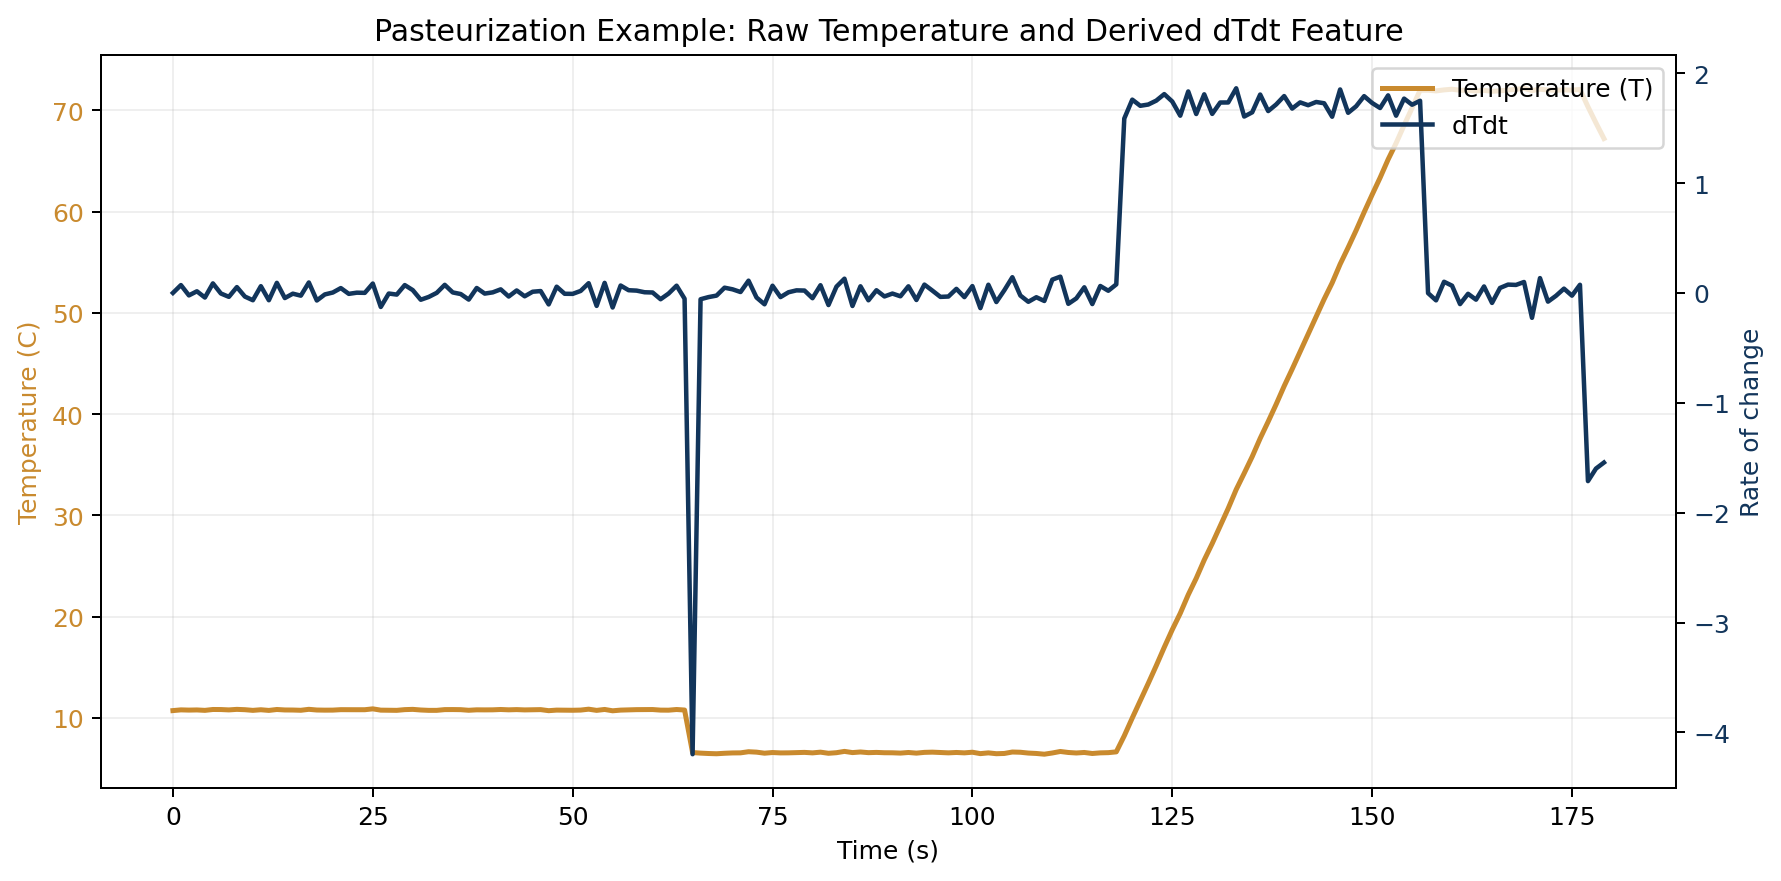
\includegraphics[height=0.72\textheight]{images/class04_pasteurization_dt_plot.png}

{\scriptsize In `pasteurization/synth_sensors.py`, `dTdt` is derived from the temperature time series to expose heating and cooling behavior directly.}
\coursefooter
\end{frame}

\begin{frame}{Spectral and signal data}
\begin{itemize}
\item A signal is a time series sampled densely enough that its frequency content becomes meaningful: audio, vibration, or high-rate sensor traces.
\item The Fourier transform (FFT) re-expresses a signal as a sum of frequencies instead of a sequence of amplitudes over time.
\item Audio pipelines commonly frame the signal into short overlapping windows and summarize each window (for example with MFCC features) before any modeling.
\item This repository has no dedicated audio dataset; we reason about it conceptually and connect it to the pasteurization temperature trace, which is itself a densely sampled physical signal.
\end{itemize}
\coursefooter
\end{frame}

\begin{frame}{Image data}
\begin{itemize}
\item An image is a 2D (or 3D, with color channels) grid of pixel intensities, not a table of independent variables.
\item Spatial locality matters: a pixel is strongly related to its immediate neighbors, which is why convolution-based methods exist.
\item There is no natural ``row order'' the way there is in tabular or time series data; the structure is spatial, not sequential.
\item This repository has no image dataset either; it is included here so the taxonomy is complete before we discuss encoding and representation next class.
\end{itemize}
\coursefooter
\end{frame}

\begin{frame}{What breaks when the data type is ignored}
\begin{tabularx}{\textwidth}{>{\bfseries}l X}
Data type & What a naive tabular treatment breaks \\
\toprule
Time series & Random train/test splits leak future information into the past. \\
Spectral / signal & Raw amplitude values hide the periodic structure that actually matters. \\
Image & Flattening pixels into columns destroys spatial neighborhoods. \\
\bottomrule
\end{tabularx}
\coursefooter
\end{frame}

\begin{frame}{From data type to system design}
\centering
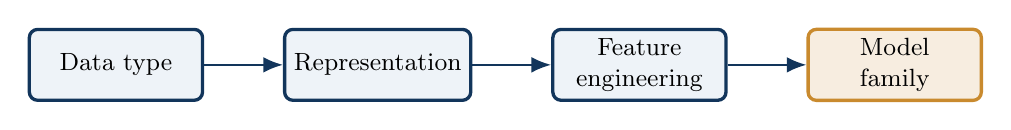
\begin{tikzpicture}[node distance=1cm and 1cm]
\node[flowbox] (type) {Data type};
\node[flowbox, right=of type] (rep) {Representation};
\node[flowbox, right=of rep] (feat) {Feature\\engineering};
\node[accentbox, right=of feat] (model) {Model\\family};
\draw[arrow] (type) -- (rep);
\draw[arrow] (rep) -- (feat);
\draw[arrow] (feat) -- (model);
\end{tikzpicture}
\vspace{0.5em}
\begin{itemize}
\item Every arrow in this chain is a later class: representation and encoding (Class 14), feature engineering (Class 15), and modeling (Class 16--17).
\item Getting the first box wrong quietly biases everything downstream.
\end{itemize}
\coursefooter
\end{frame}

\begin{frame}{Repository connections}
\repoactivity{
\begin{itemize}
\item `Credit_Card_Fraud_Detection_Solution.ipynb` and `streamlit/modeling.py` are the tabular example: one row per transaction.
\item `pasteurization/synth_sensors.py` is the time series and signal example: seven sensors sampled once per second across a batch lifecycle.
\item `pasteurization/serving.py` turns that same time series into a live stream, which is the practical lab in Class 19.
\end{itemize}
}
\coursefooter
\end{frame}

\begin{frame}{Common mistakes when data type is ignored}
\begin{itemize}
\item Treating a time-ordered sensor log as an i.i.d. table and shuffling it before splitting.
\item Applying tabular feature-importance tools to raw pixel columns and expecting them to mean anything.
\item Ignoring sampling rate: a signal sampled too slowly cannot represent the frequencies you care about.
\item Forgetting that ``more data'' is not the same as ``more independent observations'' in time series and signals.
\end{itemize}
\coursefooter
\end{frame}

\begin{frame}{Discussion prompt}
\begin{block}{Question}
The pasteurization sensors are logged into a table with one row per second. Is that table tabular data, time series data, or both?
\end{block}
\begin{itemize}
\item The goal is to separate storage format (a table) from data semantics (temporal dependency).
\item This sets up the encoding and representation discussion in Class 14.
\end{itemize}
\coursefooter
\end{frame}

\begin{frame}{Papers and materials}
\readinglist{
\href{https://www.tandfonline.com/doi/abs/10.1080/01621459.1977.10480935}{Tukey (1977), Exploratory Data Analysis};\
\href{https://link.springer.com/book/10.1007/978-0-387-45528-0}{Bishop, Pattern Recognition and Machine Learning};\
\href{https://www.oreilly.com/library/view/designing-machine-learning/9781098107956/}{Chip Huyen, Designing Machine Learning Systems};\
\href{https://pandas.pydata.org/docs/getting_started/overview.html}{pandas overview}.
}
\coursefooter
\end{frame}

\classclosingframe
{\begin{itemize}
\item Data has an intrinsic type: tabular, time series, spectral/signal, or image, each with different structural assumptions.
\item The fraud case is our tabular anchor; the pasteurization case is our time series and signal anchor.
\item Getting the data type right is a precondition for every later step, not an optional first slide.
\end{itemize}}
{Before writing any preprocessing code for a project, teams should state explicitly which data type each of their inputs is.}
{Class 14 asks how each data type is organized (structured, semi-structured, unstructured) and how we turn it into numbers through encoding and dimensionality reduction.}
{Understanding data type is the first of four steps: type, representation, features, model.}

\end{document}
